\documentclass[10pt,a4paper]{article}
\usepackage[margin=20mm]{geometry}
\usepackage[T1]{fontenc}
\usepackage{lmodern}
\usepackage{microtype}
\usepackage{graphicx}
\usepackage{booktabs}
\usepackage{amsmath}
\usepackage{xcolor}
\usepackage[colorlinks=true,urlcolor=blue!55!black,linkcolor=blue!55!black]{hyperref}
\setlength{\parindent}{0pt}
\setlength{\parskip}{4pt}
\setlength{\textfloatsep}{9pt}
\setlength{\intextsep}{9pt}
\renewcommand{\refname}{References}
\newcommand{\Ntotal}{820}
\newcommand{\Ntrain}{670}
\newcommand{\Ntest}{150}
\newcommand{\Nsources}{1}
\newcommand{\Ngroups}{455}
\newcommand{\NtrainGroups}{364}
\newcommand{\NtestGroups}{91}
\newcommand{\ChosenModel}{XGBoost}
\newcommand{\ResultsRows}{%
Ridge & 11.87 $\pm$ 1.35 & 0.084 & 12.98 & 9.67 \\
Random Forest & 7.12 $\pm$ 1.12 & 0.713 & 7.27 & 4.67 \\
XGBoost & 7.00 $\pm$ 1.10 & 0.740 & 6.92 & 4.29 \\
}

\newcommand{\RepositoryLink}{\url{https://github.com/yhzhangchn/CV7001-ML}}


\begin{document}
\begin{center}
{\Large\bfseries Prediction of Geopolymer Concrete\\Compressive Strength\par}
\vspace{5pt}
{\normalsize ZHANG YUNHAN \quad G2509929H\par}
\vspace{2pt}
{\small CV7001 Scientific Computational Methods \quad | \quad ML Mini-Project\par}
{\small GitHub: \RepositoryLink\par}
\end{center}
\vspace{-6pt}

\section{Problem and Motivation}
This project predicts the compressive strength of geopolymer concrete from mixture composition, curing conditions and specimen age. Such predictions can help compare mixtures during material selection. I used a public dataset to train Ridge regression, Random Forest and XGBoost, then compared their accuracy on withheld mixtures.

\section{Dataset and Method}
Aravind-Unni's GPC Dataset contains \Ntotal{} records, 13 predictors and measured compressive strength in MPa~\cite{data}. All 820 records were included.

I selected ten inputs before training: seven material amounts (NaOH, sodium silicate, GGBFS, fly ash, extra water, fine aggregate and coarse aggregate, in kg/m$^3$), NaOH molarity, curing temperature and specimen age. Molarity and temperature distinguish records with the same material amounts tested under different preparation conditions.

A base composition is defined by the seven material amounts rounded to eight decimals, giving \Ngroups{} groups. Records with the same composition stay together across ages and preparation conditions. A grouped 80:20 split (seed 42) reserves \NtestGroups{} groups/\Ntest{} records for testing and leaves \NtrainGroups{} groups/\Ntrain{} records for development. The test set contains 20\% of groups and 18.3\% of records.

Five-fold \texttt{GroupKFold} evaluates the development data (shuffle seed 42). Ridge uses standardisation within each training fold and $\alpha=1$~\cite{sklearn}. Random Forest has 300 trees and maximum depth 8. XGBoost has 300 trees, depth 6, learning rate 0.05, and row/column sampling ratios of 0.8~\cite{xgb}. I selected the lowest-CV-RMSE model with these fixed settings. All models use identical folds and test records. For the selected model, permutation importance measures the increase in validation RMSE after shuffling each input ten times within each development fold.

\section{Results and Discussion}
\begin{table}[ht]
\centering
\small
\caption{Development CV and holdout performance.}
\begin{tabular*}{\linewidth}{@{}l@{\extracolsep{\fill}}cccc@{}}
\toprule
Model & CV RMSE & Test $R^2$ & Test RMSE & Test MAE \\
\midrule
\ResultsRows
\bottomrule
\end{tabular*}
\par\vspace{3pt}
{\footnotesize\raggedright\textit{Note:} Errors are in MPa. CV RMSE reports the five-fold mean $\pm$ sample SD.\par}
\end{table}

XGBoost gives the lowest CV RMSE and a test $R^2=0.740$, RMSE $=6.92$ MPa and MAE $=4.29$ MPa. Its test RMSE is 46.7\% lower than Ridge's $12.98$ MPa, but only 4.8\% lower than Random Forest's $7.27$ MPa. The main gain therefore comes from using a nonlinear tree ensemble; the difference between the two ensembles is smaller. XGBoost's training RMSE of $1.97$ MPa rises to $6.92$ MPa for unseen base compositions.

\begin{figure}[ht]
\centering
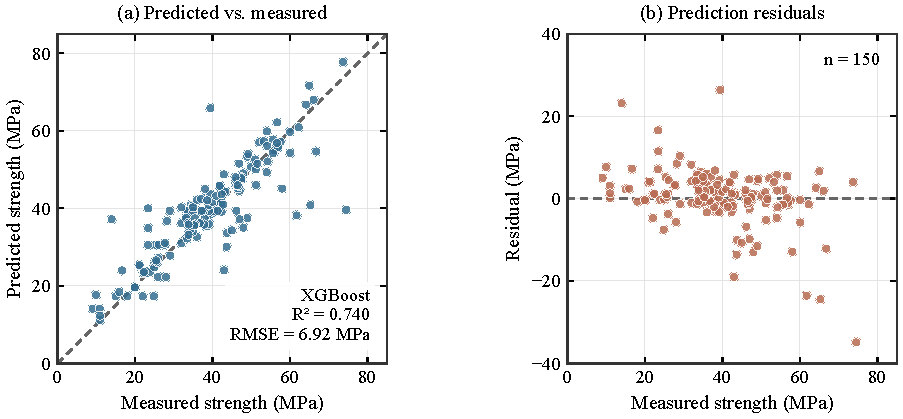
\includegraphics[width=\linewidth]{figures/heldout_predictions.pdf}
\caption{XGBoost predictions for the 150 held-out observations. Dashed lines denote perfect agreement (left) and zero error (right). Errors are predicted minus measured strength.}
\end{figure}

Of the 150 test predictions, 109 (72.7\%) fall within 5 MPa of the measurements and 134 (89.3\%) within 10 MPa. Table~\ref{tab:bands} separates the errors by measured strength. MAE is lowest for strengths from 20 to below 60 MPa ($3.67$ MPa). Below 20 MPa, the model overpredicts by $5.16$ MPa on average; at 60 MPa and above, it underpredicts by $7.95$ MPa. These opposing biases show a tendency toward intermediate strengths. For example, one 74.50 MPa observation is predicted as 39.60 MPa.

\begin{table}[ht]
\centering
\small
\caption{XGBoost errors by measured strength.}
\label{tab:bands}
\begin{tabular*}{\linewidth}{@{}l@{\extracolsep{\fill}}rrr@{}}
\toprule
Strength (MPa) & Test records & MAE (MPa) & Mean error (MPa) \\
\midrule
$<20$ & 10 & 5.31 & +5.16 \\
$20$--$<60$ & 129 & 3.67 & +0.77 \\
$\geq60$ & 11 & 10.69 & $-7.95$ \\
\bottomrule
\end{tabular*}
\par\vspace{3pt}
{\footnotesize\raggedright\textit{Note:} Mean error is predicted minus measured strength.\par}
\end{table}

\begin{minipage}{\linewidth}
The development-fold permutation analysis ranks GGBFS content and NaOH molarity first: shuffling them increases RMSE by $7.52$ and $7.16$ MPa, respectively. Curing temperature follows at $2.52$ MPa. The model therefore relies most on slag dosage and activator concentration, with curing temperature providing additional predictive information.
\end{minipage}

\section{Conclusions and Reflection}
With ten inputs, the selected XGBoost model reduces test RMSE from $12.98$ to $6.92$ MPa relative to Ridge. Slag content, NaOH concentration and curing temperature are the leading predictors in the development analysis. Accuracy is highest from 20 to below 60 MPa; high-strength mixtures are the clearest weakness, with MAE nearly three times as large. Only 52 of 670 development records reach 60 MPa, making additional high-strength data a targeted next step.

\section*{Reproducibility and Disclosures}
The project includes code, data and a README with training and prediction instructions.

Generative AI assisted with code editing, verification and report drafting.

\begin{thebibliography}{9}\setlength{\itemsep}{0pt}
\bibitem{data} Aravind-Unni. \emph{GPC Dataset}. \url{https://github.com/Aravind-Unni/GPC-Dataset}.
\bibitem{sklearn} F. Pedregosa et al. Scikit-learn: Machine learning in Python. \emph{JMLR}, 12:2825--2830, 2011. \url{https://jmlr.org/papers/v12/pedregosa11a.html}.
\bibitem{xgb} T. Chen and C. Guestrin. XGBoost: A scalable tree boosting system. \emph{KDD}, 2016. \url{https://doi.org/10.1145/2939672.2939785}.
\end{thebibliography}
\end{document}
